\chapter{Implementation and evaluation}
\label{chap:impl}


This chapter is dedicated to implementing the \textit{RRMGreedy++} algorithm described in Section \ref{chap:research:sec:rrmv2}, as well as other algorithms described in Section \ref{chap:lr} and comparing their performance. In this study, I use the ns-3 discrete-event simulation framework for implementing and evaluating different RRM algorithms.

The chapter is organized as follows:
\begin{itemize}
    \item Section \ref{chap:impl:sec:simulation_method} describes the simulation methodology used to evaluate the performance of RRM algorithms, and the process of adjusting ns-3 to needs of running and evaluating RRM algorithms;
    \item Section \ref{chap:impl:sec:implementation} describes my implementation of \textit{RRMGreedy++}, \textit{RRMGreedy}, and \textit{Least Congested Channel Search} (LCCS) algorithms in ns-3;
    \item Section \ref{chap:impl:sec:eval} presents the results of the simulation study, comparing RRM algorithms: RRMv2, RRMGreedy, and Least Congested Channel Search (LCCS), in terms of network throughput and interference;
    \item Finally, Section \ref{chap:impl:sec:conclusion} concludes the chapter with a summary of the results and a discussion of the implications of the study.

\end{itemize}

\section{Simulation methodology}
\label{chap:impl:sec:simulation_method}
In this study, I implement LCCS, RRMGreedy and RRMGreedy++ algorithms in ns-3 simulator to have a scalable, flexible (from dozens to hundreds of APs), and reproducible (unlike real-world testbeds) way to evaluate performance of different RRM algorithms under different conditions.

\subsection{RRM support in ns-3}
The ns-3 simulator is a comprehensive tool for research in computer networks, modeling each layer of the OSI model and providing simulations for wired and wireless communication technologies and protocols, including LTE, Wi-Fi, and Ethernet. Nevertheless, despite its extensive capabilities, there is a limited support for simulating RRM algorithms.

In addressing this gap, \cite{bharadwajSimulationFrameworkRadio2017} introduced an RRM framework that employs an additional radio interface, termed a "scan interface." Unlike the standard "data interface" used for communication, the scan interface periodically surveys a specified set of channels. It operates in \textit{promiscuous mode}, allowing it to capture all frames and physical layer headers intercepted by the data interface. Thus, scan interface is able to record Received Signal Strength Indicator (RSSI) values from transmissions between devices that the data interface is engaged with. This resembles scanning radios found in high-end Cisco access points. Unlike the Cisco solution, this scanning interface, however, can be used both with stations and access points.

However, this model presents several deviations from real-world scenarios:
\begin{itemize}
    \item Most hardware, apart from high-end Cisco models, lacks a dedicated scanning interface, leading to scanning activities disrupting normal data exchanges. This interruption, referred to as \textit{"dead time,"} denotes periods when scanning supersedes the standard operation of an Access Point (AP);
    \item For mobile devices, scanning capabilities are significantly restricted to avoid draining the battery;
    \item The \texttt{RriModule} code and its associated examples, designed for ns-3 version 3.20, are incompatible with the current ns-3 version 3.40 API and the legacy Waf build system. As a part of my contribution, I have refactored the original code to align with the latest ns-3 version 3.41 API, specifically updating the \texttt{RriModule} to integrate with the latest \texttt{WifiMac} ns-3 API and the CMake build system. This adaptation ensures the compatibility and execution on the newest ns-3 version. The modified source code is publicly available on GitHub.
\end{itemize}

\subsection{Providing scanning capabilities in ns-3}
\label{chap:impl:sec:simulation_method:subsec:scanning}

In real-world scenarios, wireless access points implement scanning by setting the wireless adapter to monitor mode and sequentially switching to each channel that requires scanning. Although direct support for monitor mode is absent in ns-3, a comparable functionality can be simulated using the \texttt{MonitorSnifferRx} event source. Subscribing to such events allows for the interception of all frames that the physical layer of the access point can receive and demodulate, even if those frames would be normally discarded as not intended for the current AP \cite{Ns3AllTraceSources}. However, this method does not exclude standard operations of an access point; the AP still continues to receive and transmit frames. This is not the case in actual access points, where operating monitor mode is mutually exclusive to AP's normal operation. To achieve nearly the same result, my approach prevents the AP from transmitting frames during the scanning period.

Based on the consideration above, I designed an external \texttt{Scanner} class that encloses \texttt{WifiNetDev} of access point nodes. Scanner can be used on arbitrary AP node to give it background scanning capabilities.
The \texttt{LCCScanner} class is invoked on \texttt{MonitorSnifferRx} event, simulating receiving frames in monitor mode. For each received frame, if this frame comes from an AP (either a beacon frame or has \texttt{FromDs} flag set to 1), it is added to \texttt{knownAps} table.
If scheduled, Scanner periodically switches to other channels for specified \textit{channel dwell period}, listening for frames. To reduce disruptions in AP's regular BSS operation, the AP returns to its operating channel after performing scanning on one channel, proceeding to scan next channel after a specified \textit{scan interval}. Such behavior is also implemented in Cisco access points \cite{ciscoRadioResourceManagement}.
Based on this frame capture, Scanner builds a table of known APs, containing information such as BSSID, operating channel, RSSI and SNR levels, and the number of client stations associated with the AP. This table is then used by RRM algorithms to make decisions on channel and power adjustments.

Another limitation I have encountered during the implementation is the lack of channel switching logic for unassociated stations performing scans to discover an access point for association. In practical scenarios, stations scan all available channels within the operating bands to discover access points, however, as of the latest ns-3 version 3.41, released in February 2024, such functionality is absent in \texttt{ns3::StaWifiMac} class, which implements the logic for STA (stations) operation. Consequently, ns-3 Wi-Fi stations can only scan for APs present on the current operating channel. For instance, if both AP and stations are on channel 1, and the AP shifts to channel 6, the stations remain unable to scan beyond channel 1 to ascertain the AP's new location on channel 6. To address this problem, I have implemented a custom scanning logic, allowing stations to scan all available channels in its operating band. This amendment is available in the modified source code on GitHub.


\section{Implementation}
\label{chap:impl:sec:implementation}
This section provides an implementation of various Radio Resource Management (RRM) strategies, utilizing the ns-3 discrete-event simulation framework.

\subsection{Least Congested Channel Search (LCCS)}
\label{chap:impl:sec:implementation:lccs}
LCCS is a patented local per-cell algorithm described in \cite{achantaMethodApparatusLeast2006}. Essentially, it breaks down to estimating the interference level on each channel and selecting the least congested one. The algorithm is implemented in practically every home Wi-Fi router. The algorithm is simple, but it does not coordinate channel selection across multiple APs, which is crucial for performance in large-scale deployments.
In my ns-3 LCCS implementation, I introduce \texttt{LCCSAlgo} class. Method \texttt{LCCSAlgo::Decide} perform LCCS channel switching decision and is invoked as a callback from \texttt{Scanner} class, described in Section \ref{chap:impl:sec:simulation_method:subsec:scanning}.
Algorithm \ref{alg:lccs} describes my LCCS implementation.

\begin{algorithm}[H]
\label{alg:lccs}
\caption{Least Congested Channel Search}
\DontPrintSemicolon
\SetAlgoLined
\SetKwInput{KwInput}{Input}
\SetKwInput{KwOutput}{Output}
\SetKwFunction{FMain}{LCCSAlgo::Decide}
\SetKwProg{Fn}{Function}{:}{}
\KwInput{\textit{scanningAP}: AP that invoked the LCCS call}
\KwOutput{\textit{newChannel}: new channel for AP to switch to}

\Fn{\FMain{scanningAP}}{
    metrics $\gets$ table that maps each channel to its metric, initially 0 for each channel\;

    \ForEach{apEntry in scanningAP.knownAps}{
        metrics[apEntry.channel] $\gets$ \newline metric[apEntry.channel] + 1 + 10 $\times$ size(apEntry.clients)\;
    }
    newChannel $\gets$ argmin(metrics)\;
    return newChannel\;
}
\end{algorithm}

Note that I intended to keep the algorithm simple to conform closer with the original flow described in \cite{achantaMethodApparatusLeast2006}. Real-world LCCS implementation tend to use more sophisticated heuristics and metrics to estimate channel congestion.

\subsection{RRMGreedy}
\label{chap:impl:sec:implementation:rrmgreedy}
RRMGreedy is a centralized super-cell algorithm used by a leading Russian telecommunications vendor, described and analyzed in Chapter \ref{sec:baseline}.
Implementing RRMGreedy in ns-3 requires a centralized entity to gather data from all APs and perform computations. I introduce \texttt{RRMGreedyAlgo} class, which is responsible for collecting data from all APs and making decisions on channel and power adjustments.
Unlike LCCS, RRMGreedy is not invoked by APs due to its centralized nature. Since the original RRMGreedy does not requests scanning data directly from APs, but rather queries the database to which APs send periodical reports, I aimed to achieve similar behavior.
Thus, \texttt{RRMGreedyAlgo::AddApScandata} is set as a callback for each \texttt{Scanner} instance in an RRM group to submit the individual scanning results to RRMGreedy after every full scanning cycle. Each \texttt{scandata} item has a timestamp, and RRMGreedy does not accept scanning data older than \textit{scandataStaleTime} parameter (in seconds). Callback method \texttt{RRMGreedyAlgo::Decide} is invoked by the simulation scheduler at regular intervals to perform RRM decisions.
Channel Planning is implemented using the same approach found in LCCS. However, implementing TPC was a considerable challenge, since ns-3 does not support setting AP's transmit power directly. To address this issue, I manipulated starting and ending Tx power levels of phy layer of a WifiNetDevice of an AP node.

\subsection{RRMGreedy++}
\label{chap:impl:sec:implementation:rrmv2}

TBD

\section{Evaluation}
\label{chap:impl:sec:eval}
To evaluate the performance of RRM algorithms, I have conducted a series of test cases for simulations in ns-3. These test case share several common parameters that are fixed (\autoref{table:fifsimulation_params}); each test case is also characterized by a set of unique parameters (\autoref{table:eval_testcases})
\subsection{Simulation settings}
\begin{longtable}{|c|c|}
\caption[Simulation Parameters]{Fixed Simulation Parameters} \label{table:fifsimulation_params} \\
\hline
\textbf{Parameter} & \textbf{Value} \\
\hline
\endfirsthead
\multicolumn{2}{@{}l}{} \\
\hline
\endhead
\hline
Frequency band & 2.4 GHz \\
\hline
IEEE 802.11 amendment & 802.11n \\
\hline
Data rate & 54 Mbit/s \\
\hline
Channel width & 20 MHz \\
\hline
\end{longtable}

% \begin{itemize}
%     \item \textbf{Test Case 1:}
%     \begin{itemize}
%         \item Number of APs: 3;
%         \item Number of STAs: 7;
%         \item STA allocations by AP: $\{3, 2, 2\}$;
%         \item Initial channel allocations by AP: $\{1, 1, 1\}$;
%         \item Initial channel allocations on stations: all start on channel 1 and until given SSID is found;
%         \item Traffic model: each AP has at least one pair of STAs, where first STA in the pair generates UDP generating traffic as UDP client, and second echoing it back to client as UDP server;
%         \item Simulation time: 10s.
%     \end{itemize}
% \end{itemize}

\begin{longtable}{|p{6cm}|p{7cm}|}
\caption{Test Case Configurations}
\label{table:eval_testcases} \\
\hline
\multicolumn{2}{|p{8cm}|}
{\textbf{Test Case 1}} \\ \hline
\textbf{Parameter} & \textbf{Value} \\ \hline
% \multicolumn{2}{@{}l}{} \\
Number of APs & 3 \\ \hline
Number of STAs & 7 \\ \hline
Number of STA allocated for each AP & $\{3, 2, 2\}$ \\ \hline
Initial channel allocations for APs  & $\{1, 1, 1\}$ \\ \hline
Initial channel allocations for STAs & All on channel 1 \\ \hline
Traffic model  & each AP has at least one pair of STAs, where first STA in the pair generates UDP traffic as client, and second echoing it back to client as UDP server \\ \hline
Simulation time & 10s \\ \hline
Offered load per flow (Mbit/s) & 1.64 \\ \hline
\hline
\multicolumn{2}{|p{8cm}|}
{\textbf{Test Case 2}} \\ \hline
\textbf{Parameter} & \textbf{Value} \\ \hline
% \multicolumn{2}{@{}l}{} \\
Number of APs & 4 \\ \hline
Number of STAs & 7 \\ \hline
Number of STA allocated for each AP & $\{3, 2, 2, 2\}$ \\ \hline
Initial channel allocations for APs  & $\{1, 1, 1, 1\}$ \\ \hline
Initial Tx power allocations for APs  & $\{20, 20, 20, 20\}$ \\ \hline
Initial channel allocations for STAs &  All on channel 1 \\ \hline
Traffic flows and traffic model  & Each AP has at least one pair of STAs, where first STA in the pair generates UDP traffic as client, and second echoing it back to client as UDP server \\ \hline
Simulation time (seconds) & 10 \\ \hline
Offered load per flow (Mbit/s) & 1.64 \\ \hline
\hline
\multicolumn{2}{|p{8cm}|}
{\textbf{Test Case 3}} \\ \hline
\textbf{Parameter} & \textbf{Value} \\ \hline
% \multicolumn{2}{@{}l}{} \\
Number of APs & 8 \\ \hline
Number of STAs & 7 \\ \hline
Number of STA allocated for each AP & $\{3, 2, 2, 2\}$ \\ \hline
Initial channel allocations for APs  & $\{1, 1, 1, 1\}$ \\ \hline
Initial Tx power allocations for APs  & $\{20, 20, 20, 20\}$ \\ \hline
Initial channel allocations for STAs &  All on channel 1 \\ \hline
Traffic flows and traffic model  & Each AP has at least one pair of STAs, where first STA in the pair generates UDP traffic as client, and second echoing it back to client as UDP server \\ \hline
Simulation time (seconds) & 10 \\ \hline
Offered load per flow (Mbit/s) & 8.192 \\ \hline
\end{longtable}

\subsection{Metrics}
For evaluation, I collect various L3 and L2 metrics. \autoref{table:gathered_metrics} contains collected metrics, their definitions and methods to capture them using ns-3.

\begin{longtable}{|p{5cm}|p{5cm}|p{5cm}|}
\caption{Gathered Metrics}
\label{table:gathered_metrics} \\
\hline
\textbf{Metric} & \textbf{Definition} & \textbf{Means of capture}\\ \hline
Average Total WLAN Throughput & Number of L3 IPv4 Rx bytes in WLAN divided by Tx time for all nodes & ns-3 \texttt{FlowMonitor} class \\
\hline
Average L3 Delay & Average time delta between L3 (IPv4) Tx and Rx events & ns-3 \texttt{FlowMonitor} class \\
\hline
Average Total WLAN SNR (Signal-to-Noise Ratio) & Average SNR of frames received by every node in WLAN & ns-3 \texttt{MonitorSnifferRx} event \\
\hline
Average Medium Busy Time & Total time when Wi-Fi device could not transmit due to occupied medium & ns-3 \texttt{YansWifiPhy/State} trace source, notifies when Wifi PHY enters \texttt{CCA\_BUSY} state \\
\hline
Average Medium Idle Time & Total time for Wi-Fi device both not receiving and transmitting & ns-3 \texttt{YansWifiPhy/State} trace source, notifies when Wifi PHY enters \texttt{IDLE} state\\
\hline
\end{longtable}


\subsection{Results}
The results of simulation are presented below both in tabular (\autoref{table:simulation_res}) and graphical forms.

\begin{longtable}{|p{3.5cm}|p{2.5cm}|p{2cm}|p{2cm}|p{2cm}|p{2cm}|}
\caption{Simulation Results}
\label{table:simulation_res} \\
\hline
\multicolumn{6}{|p{4cm}|} {\textbf{Test Case 1}} \\ \hline
\textbf{Algorithm} & \textbf{Throughput (Mbit/s)} & \textbf{Average Delay (sec.)} & \textbf{Average Medium Busy Time (sec.)} & \textbf{Average Medium Idle Time (sec.)} & \textbf{Average SNR  (dBm)} \\ \hline
No RRM &    11.5872     &        0.0016       &       0.4295         &     0.9292  & 1\\ \hline
RRMGreedy   &   13.4000    &         0.0005      &        0.1343        &      1.2330 & 1\\ \hline
RRMGreedy++ &   13.4000    &         0.0004      &        0.1225        &      1.2486 & 1\\ \hline
\hline
\hline
\multicolumn{6}{|p{4cm}|} {\textbf{Test Case 2}} \\ \hline
\textbf{Algorithm} & \textbf{Throughput (Mbit/s)} & \textbf{Average Delay (sec.)} & \textbf{Average Medium Busy Time (sec.)} & \textbf{Average Medium Idle Time (sec.)} & \textbf{Average SNR  (dBm)} \\ \hline
No RRM          & 13.9091         & 0.0137 & 0.5268 & 0.8559 & 1 \\
\hline
RRMGreedy       &    15.8602      &       0.0007      &        0.1756      &       1.2072 & 1  \\
\hline
RRMGreedy++     &  16.5084       &      0.0007       &       0.1715        &      1.2127 & 1   \\
\hline
\hline
\multicolumn{6}{|p{4cm}|} {\textbf{Test Case 3}} \\ \hline
\textbf{Algorithm} & \textbf{Throughput (Mbit/s)} & \textbf{Average Delay (sec.)} & \textbf{Average Medium Busy Time (sec.)} & \textbf{Average Medium Idle Time (sec.)} & \textbf{Average SNR  (dBm)} \\ \hline
No RRM    &    12.7737       &      0.1900       &       1.0528        &      0.2407 & 59.0256   \\
\hline
RRMGreedy &     46.5821      &       0.0727      &        0.4341       &       0.7978 & 66.4141   \\
\hline
RRMGreedy++ &   48.6707      &       0.0405      &        0.4233       &       0.8132 & 73.4090   \\
\hline
\end{longtable}


\begin{figure}[!ht]
    \centering
    \begin{minipage}[b]{0.48\textwidth}
        \centering
        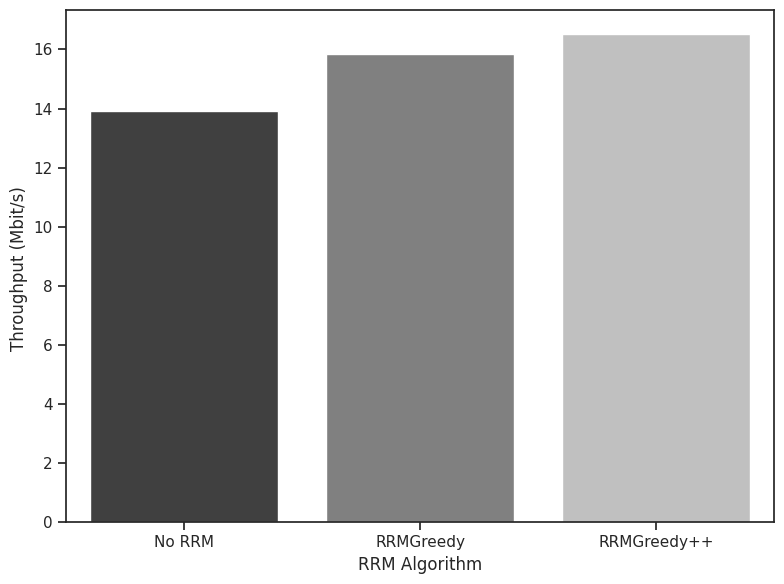
\includegraphics[width=\textwidth]{tc2_wlan_tput.png}
        \subcaption{Average total WLAN throughput}
        \label{fig:tc2:tput}
    \end{minipage}
    \hfill
    \begin{minipage}[b]{0.48\textwidth}
        \centering
        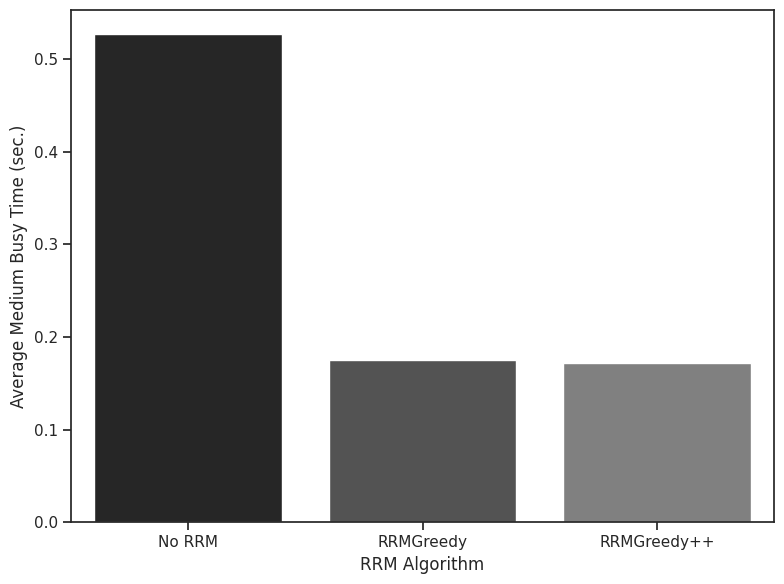
\includegraphics[width=\textwidth]{tc2_phy_busy.png}
        \subcaption{Average medium busy time}
        \label{fig:tc2:busy}
    \end{minipage}
    
    \vspace{0.1em}
    
    \begin{minipage}[b]{0.48\textwidth}
        \centering
        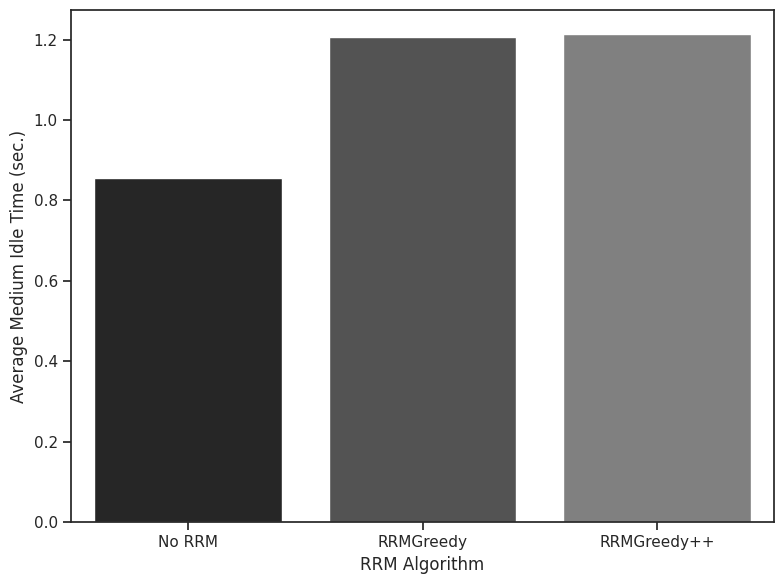
\includegraphics[width=\textwidth]{tc2_phy_idle.png}
        \subcaption{Average medium idle time}
        \label{fig:tc2:idle}
    \end{minipage}
    \hfill
    \begin{minipage}[b]{0.48\textwidth}
        \centering
        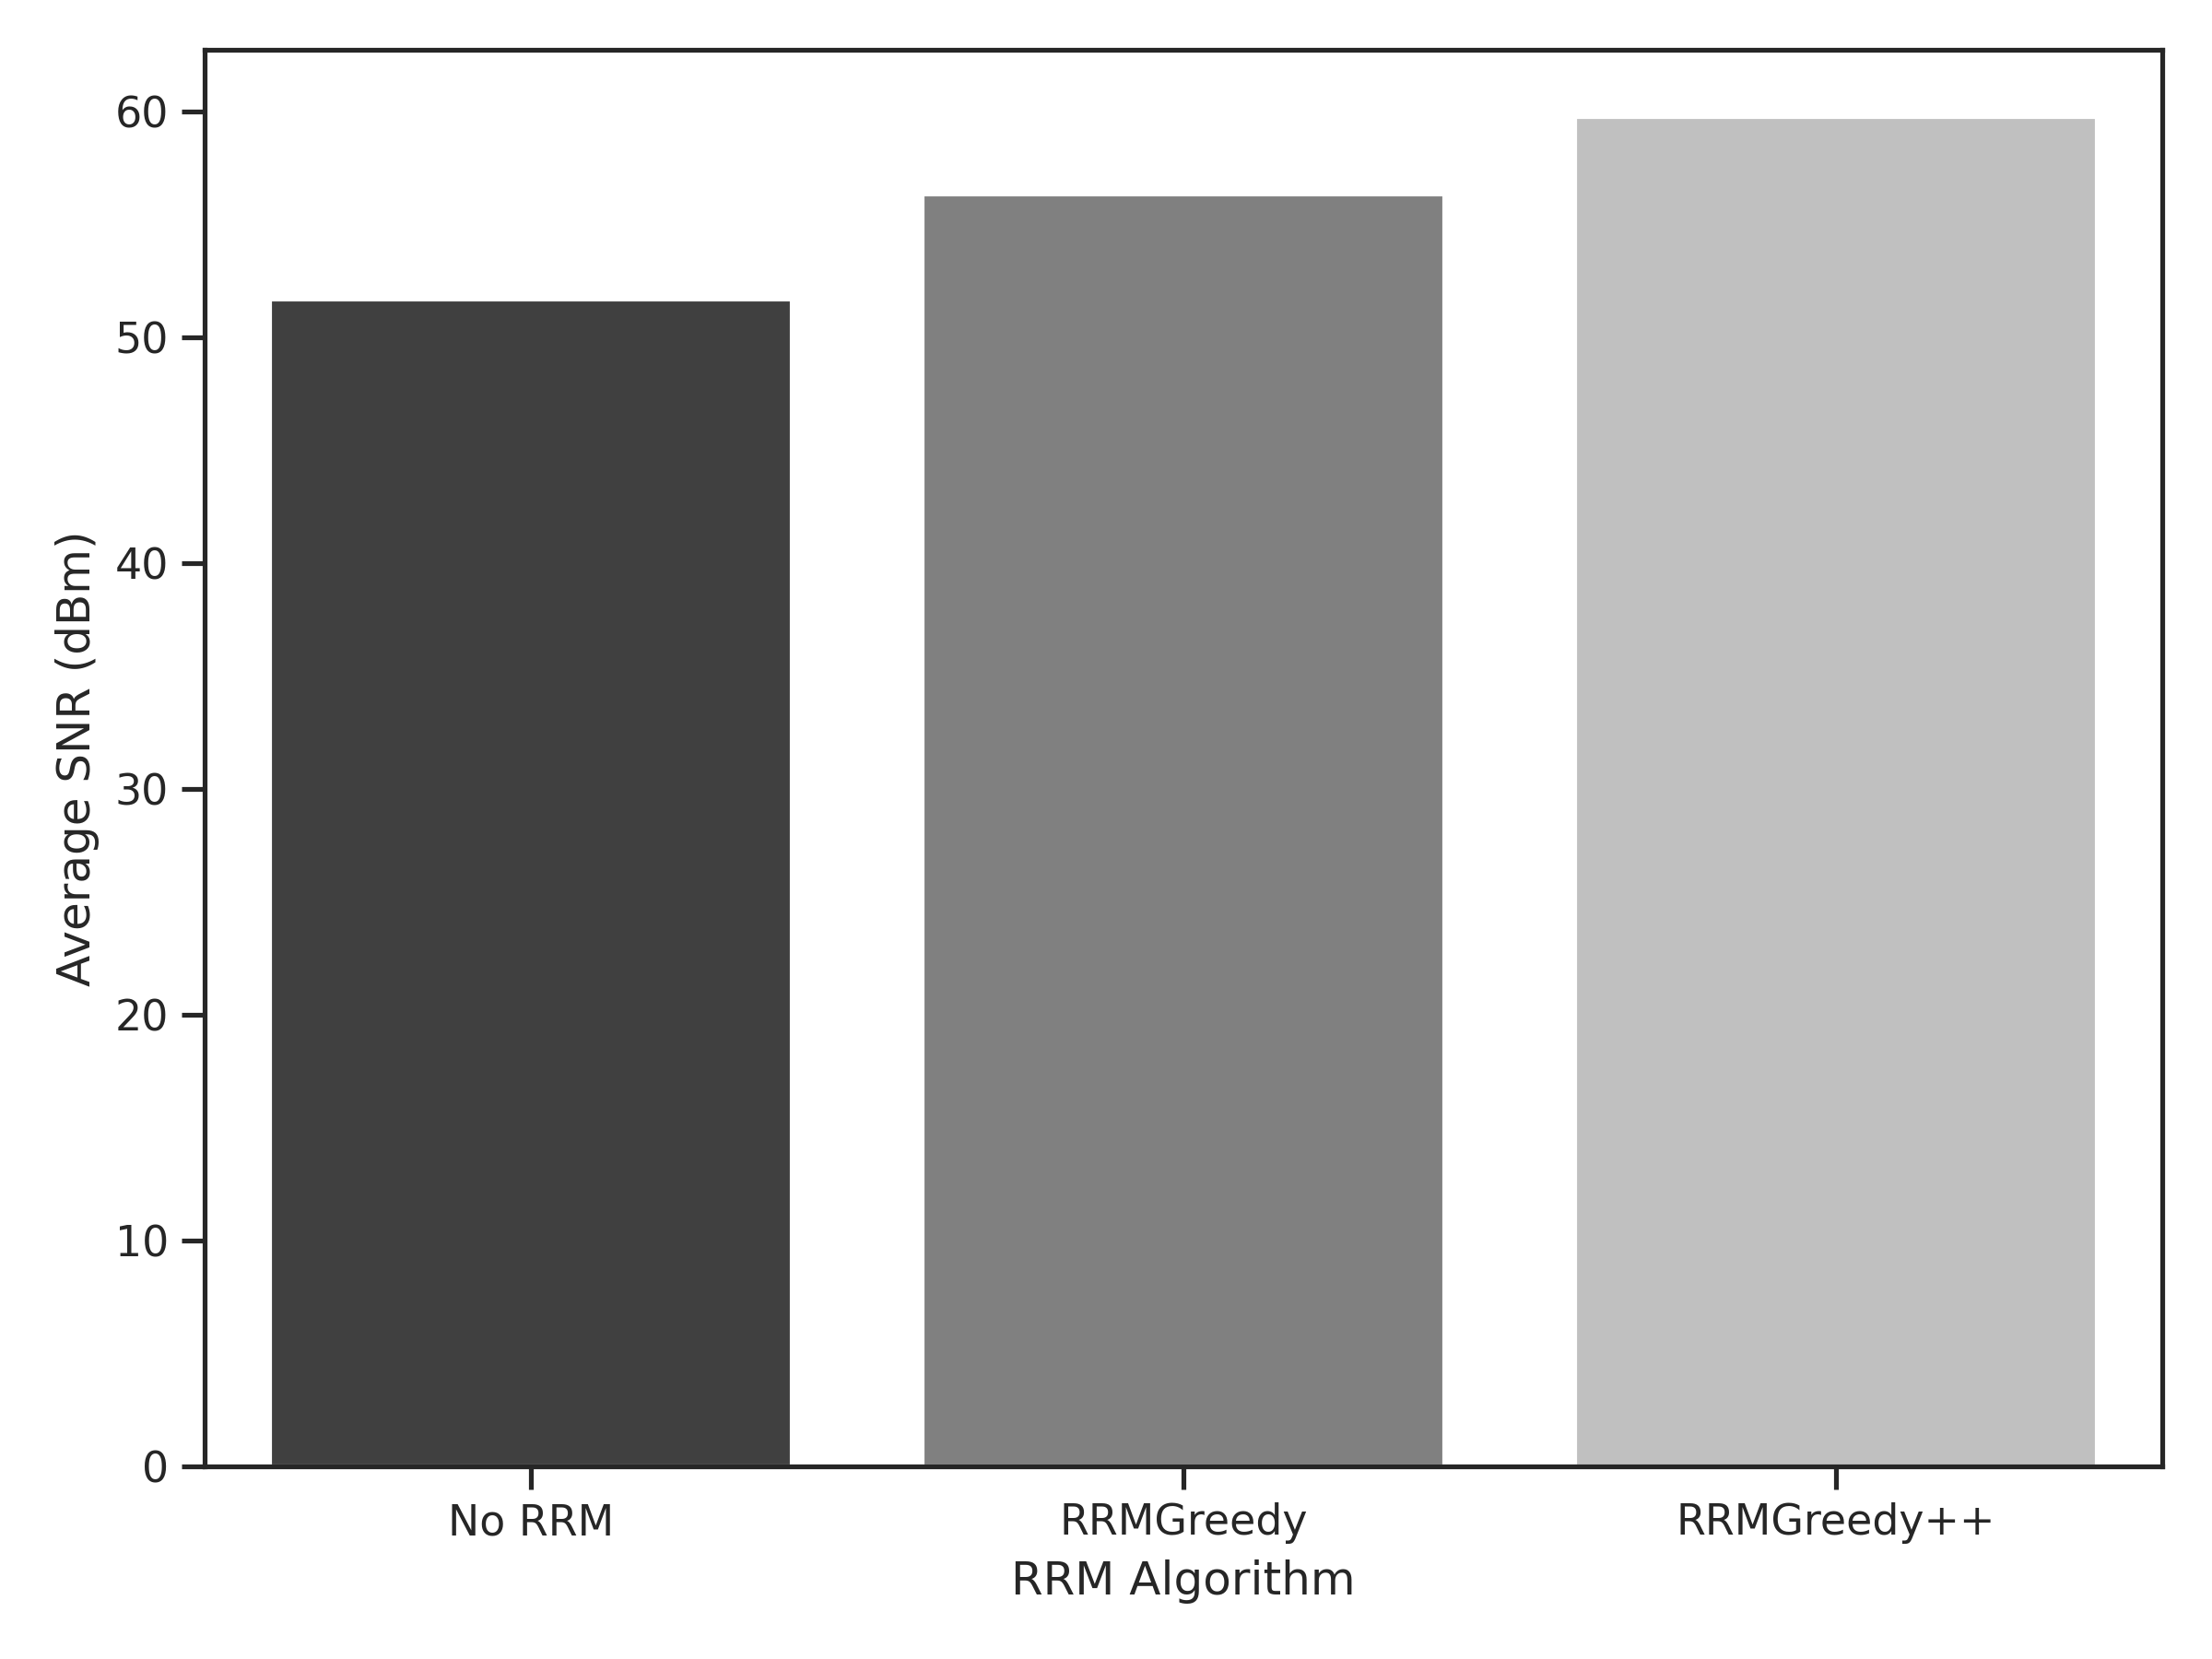
\includegraphics[width=\textwidth]{tc2_snr.png}
        \subcaption{Average SNR}
        \label{fig:tc2:snr}
    \end{minipage}
    
    \vspace{0.1em}
    
    \begin{minipage}[b]{0.48\textwidth}
        \centering
        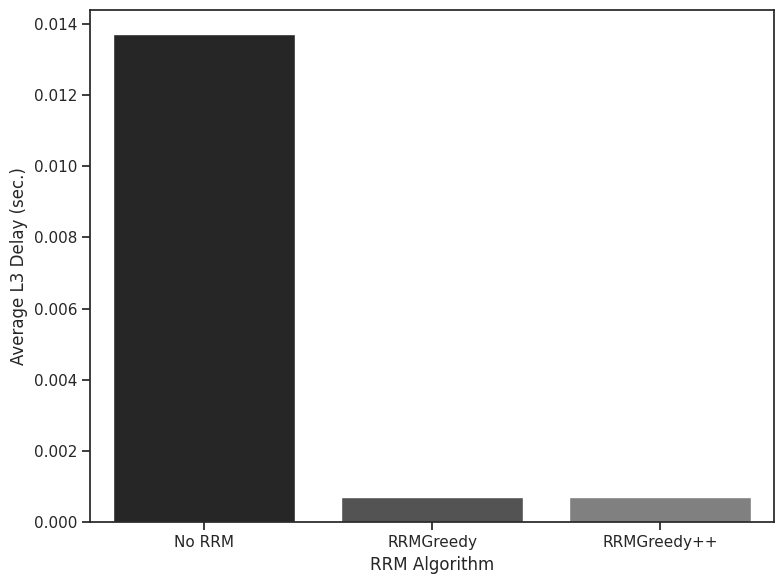
\includegraphics[width=\textwidth]{tc2_l3_delay.png}
        \subcaption{Average L3 Delay}
        \label{fig:tc2:l3delay}
    \end{minipage}
    
    \caption{Test Case 2 results}
    \label{fig:tc2:plots}
\end{figure}


\section{Conclusion}
\label{chap:impl:sec:conclusion}

Based on results, I can suggest that RRM considerably improves performance of the WLAN. That is especially evident when dealing with high offered load, as in Test Case 3. Lower Medium Busy Time and higher Medium Idle Time can be interpreted as the consequence of medium becoming less congested. Moreover, RRMGreedy and RRMGreedy++ increase total SNR of the WLAN as a result of adjusting transmission powers and switching APs to orthogonal channels.

